\documentclass[12pt, a4paper, oneside]{ctexart}
\usepackage{amsmath, amsthm, amssymb, bm, color, enumerate, float, framed, graphicx, hyperref,listings, mathrsfs, subcaption}

\title{\textbf{实验一\ 排序算法\ 实验报告}}
\author{PB18061443 江昊霖}
\date{\today}
\linespread{1.5}

\newenvironment{problem}{\begin{shaded}\stepcounter{problemnum}\par\noindent\textbf{题目\arabic{problemnum}. }}{\end{shaded}\par}
\newenvironment{solution}{\par\noindent\textbf{解答. }}{\par}

\begin{document}

\maketitle

\section{实验内容}

\begin{enumerate}
	\item 排序n个元素 ,元素为随机生成的0到$2^{15}$ − 1之间的整数, n的取值为:
$2^3, 2^6, 2^9, 2^{12}, 2^{15}, 2^{18}$。
\item 实现以下算法: 堆排序, 快速排序, 归并排序, 计数排序。
\end{enumerate}

\section{实验设备和环境}



\begin{figure*}[htbp]
\subfigure{实验装置}{	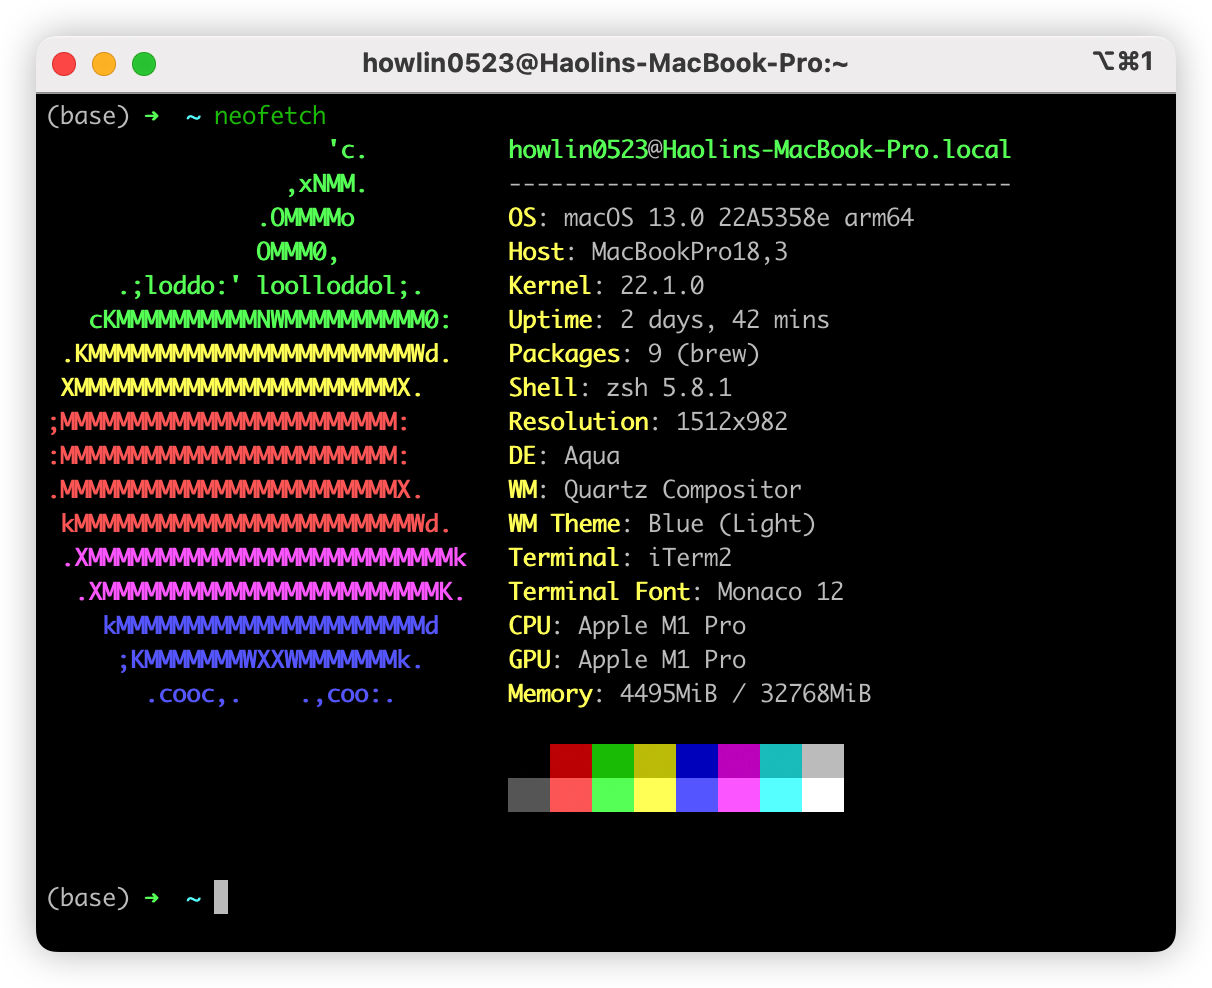
\includegraphics[width = 0.3\textwidth]{image/info.png}}
\subfigure{实验环境}{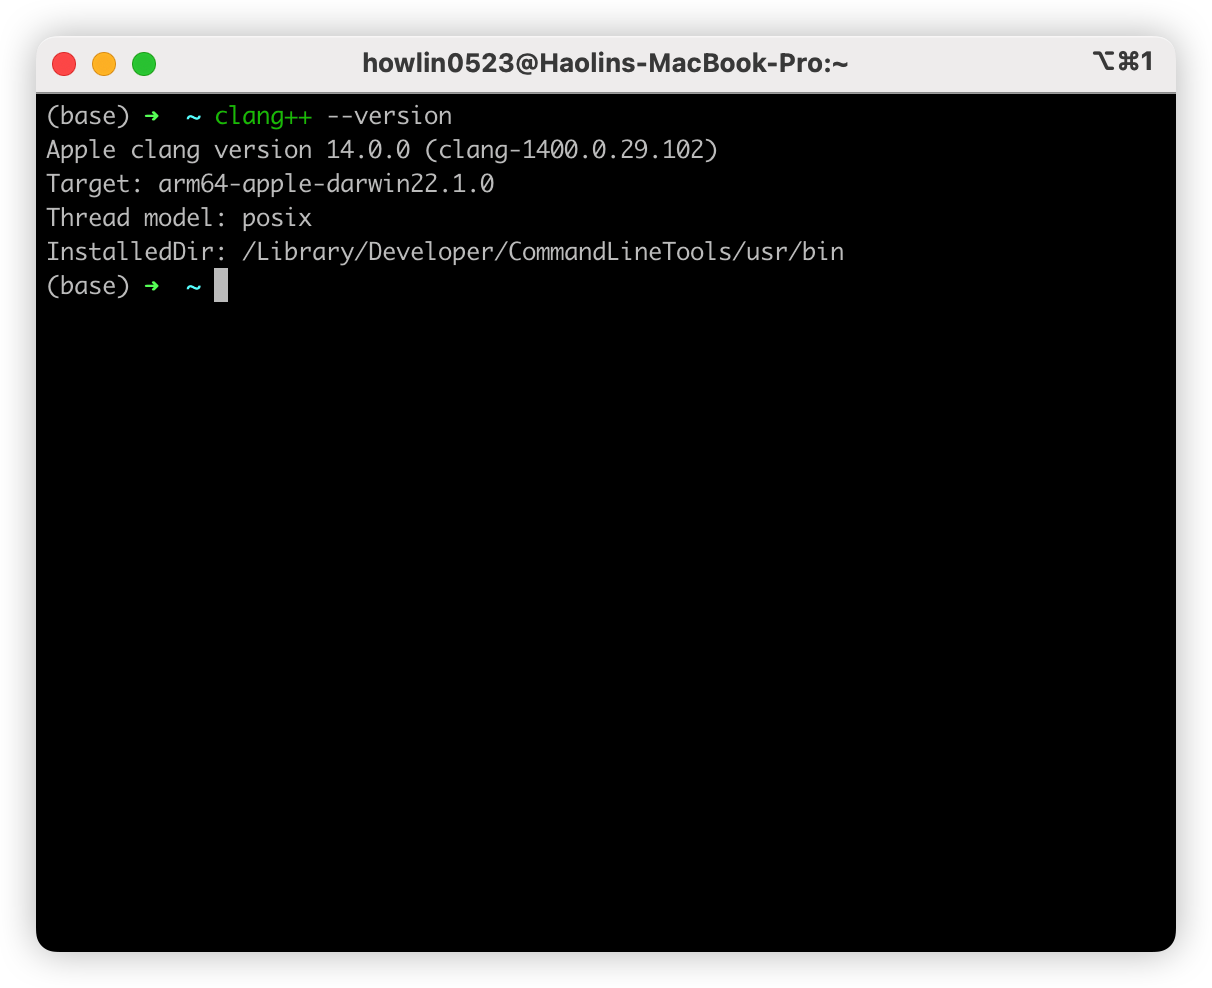
\includegraphics[width = 0.3\textwidth]{image/clang.png}}
}
\end{figure*}

\section{实验方法和步骤}

\subsection{堆排序}

\subsection{快速排序}
\subsection{ 归并排序}
\subsection{ 计数排序}
\section{实验结果与分析}







\end{document}